\ProvidesFile{ch-light-curve-simulation.tex}[Light Curve Simulation]

\chapter{Light Curve Simulation}

\section{Simulating Convex Objects}

Light curve simulation for convex geometry can be solved semi-analytically as each facet's contribution 
to the measured irradiance can be computed individually \cite{kaasalainen2001}. 
Determining whether a face is illuminated requires two horizon checks to determine visibility 
from the Sun and to the observer. For a facet $i$ at timestep $j$ these horizon checks are 
expressed by the shadowing condition $\mu_{ij}$. 

\begin{equation} \label{eq:cvx_shadow_cond}
  \mu_{ij} = \begin{cases}
    1 \text{ if } \left( \hat{O}_j \cdot \hat{n}_i \right) > 0 \text{ and } \left( \hat{S}_j \cdot \hat{n}_i \right) > 0 
	  \text{ and } \delta_{ij,\text{ss}} = 0 \text{ and } \delta_{ij,\text{os}} = 0\\
    0 \text{ otherwise } \\
  \end{cases}
\end{equation}

The unit vectors $\hat{O}$ and $\hat{S}$ point from the  center of mass of the object to the observer and Sun, respectively. 
We choose the outward-pointing facet normal unit vector $\hat{n}$ by convention for all mesh operations. 
The self-shadowing and observer-shadowing conditions, $\delta_{ij,\text{ss}}$ and $\delta_{ij,\text{os}}$, 
are always zero for convex polyhedra but are crucial for accurately simulating non-convex geometry. 
For objects with concavities, self-shadowing refers to shadows cast by an object onto itself and observer-shadowing 
refers to otherwise visible faces blocked by other portions of the geometry.

The irradiance $I$ received by the observer at timestep $j$ is the sum of the received irradiance from all facets, 
composed of specular and diffuse contributions. We express each contribution as the product of the
normalized irradiance $\hat{I}$. This can be scaled to adjust for the distance from the observer to
the object to yield the noiseless received irradiance.

\section{Simulating Non-Convex Objects}

Many existing light curve simulation methods for non-convex objects rely on ray tracing schemes like Möller and Trumbore's ray-triangle intersection algorithm \cite{moller2005,fan2020thesis}. This computation is necessarily complex as there may be significant self-shadowing at large phase angles. As a result, we cannot assume $\delta_{ij,\text{ss}} = 0$ and $\delta_{ij,\text{os}} = 0$ \cite{frueh2014,fan2020thesis}. In the absense of a bounding volume hierarchy or other techniques to reduce the number of rays cast, ray traced shadows generally require $\mathcal{O}(n^2)$ ray-triangle intersections per timestep for $n$ facets. For this reason, ray traced shadows quickly become infeasible for complex reference geometries without GPU parallelization. The limitations of ray-triangle intersections for light curve simulation is discussed at length by Frueh et al. \cite{frueh2014}.

For faster and more accurate simulated light curves, we use shadow mapping computed on the GPU. Shadow mapping is a well understood, if dated, technique in computer graphics \cite{kolivand2013}. Although modern ray traced shadowing may be more computationally efficient, shadow mapping was selected for its ease of implementation, once the inherent aliasing or `shadow acne' was addressed using standard remedies \cite{kolivand2013}. Because shadow mapping shades individual pixel fragments instead of entire facets, it offers increasing shadow quality over facetwise ray tracing as the number of mesh faces falls.

\graphicspath{{/Users/liamrobinson/Documents/msthesis/static_images/aas_2022_figs}}
\begin{figure}[!htb]
  \centering
  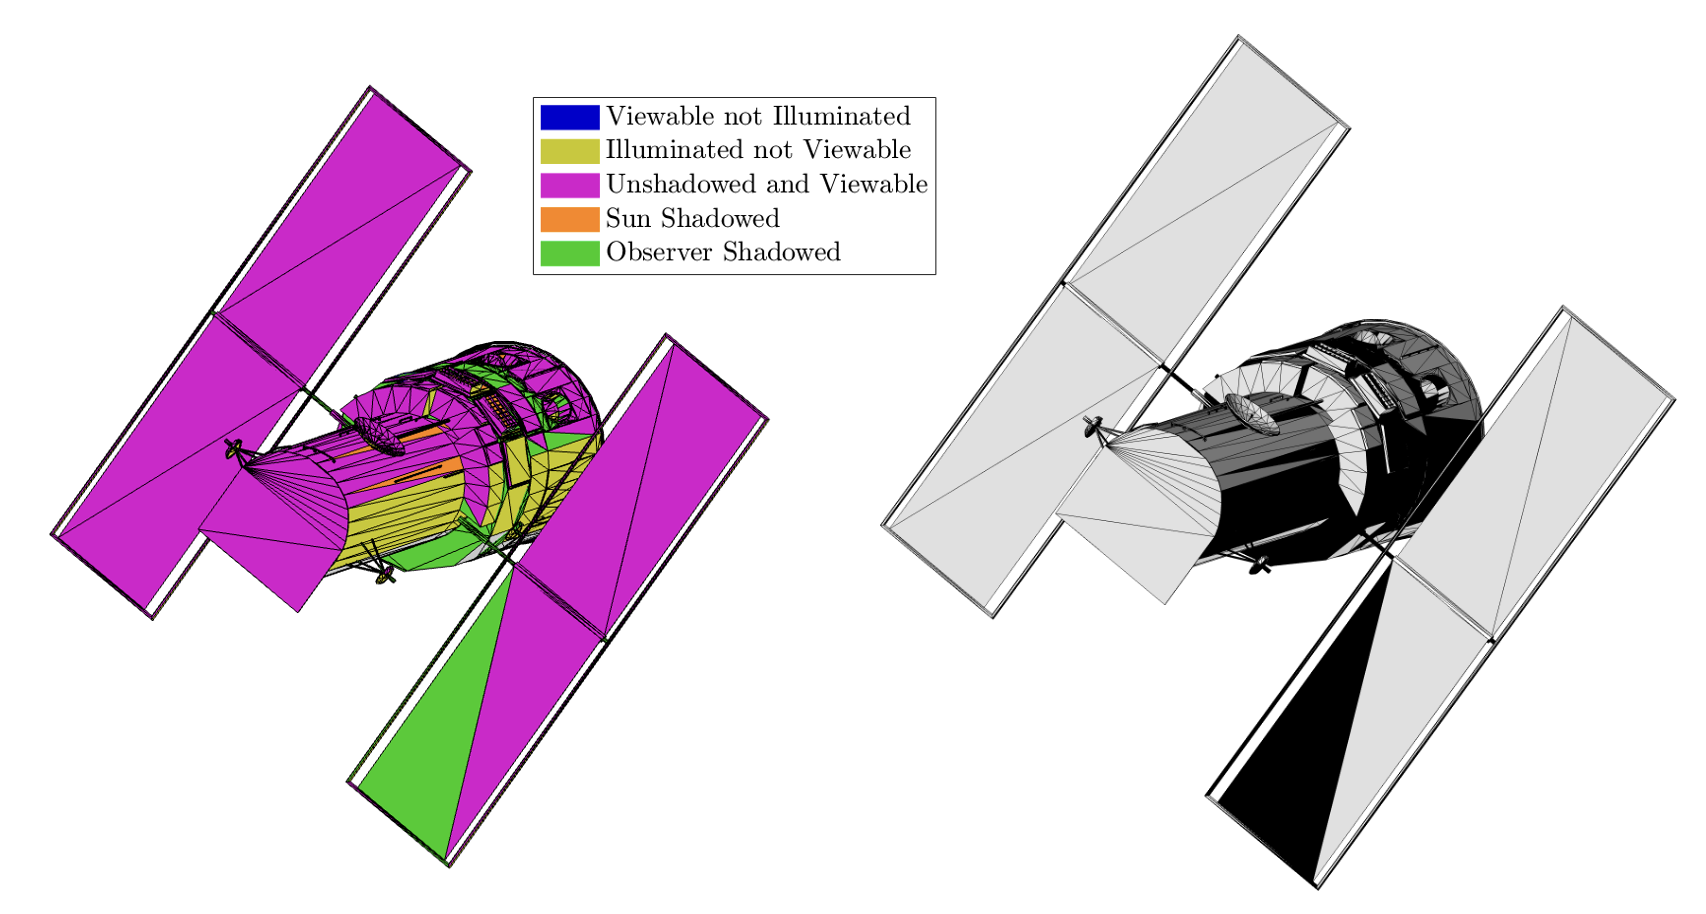
\includegraphics[width=350px]{hst_shadow_mapping/composite_hst_raytraced.png}
  \caption{Hubble Space Telescope ray traced shadow categorization and shading. Models from \cite{nasa_models}}
  \label{hst_shadows_ray}
\end{figure}

\subsection{Importance of Self-Shadowing for Human-Made Objects}

To motivate the importance of accurate shadowing computation for human-made space objects, consider the error introduced by neglecting shadows for different types of space objects. Kaasalainen and Torppa's work on asteroids reasonably assumed that shadowing was a negligible contribution to the measured light curve. Human-made objects do not afford the same luxury. Figure \ref{fig:hst_bennu_shadows} displays light curves for the asteroid Bennu and the Hubble Space Telescope with and without accurate shadows under a single-axis attitude profile with inertially fixed Sun and observer vectors. Without accurate shadowing, the light curve's magnitude and time derivatives are both dramatically effected.

\begin{figure}[!htb]
  \centering
  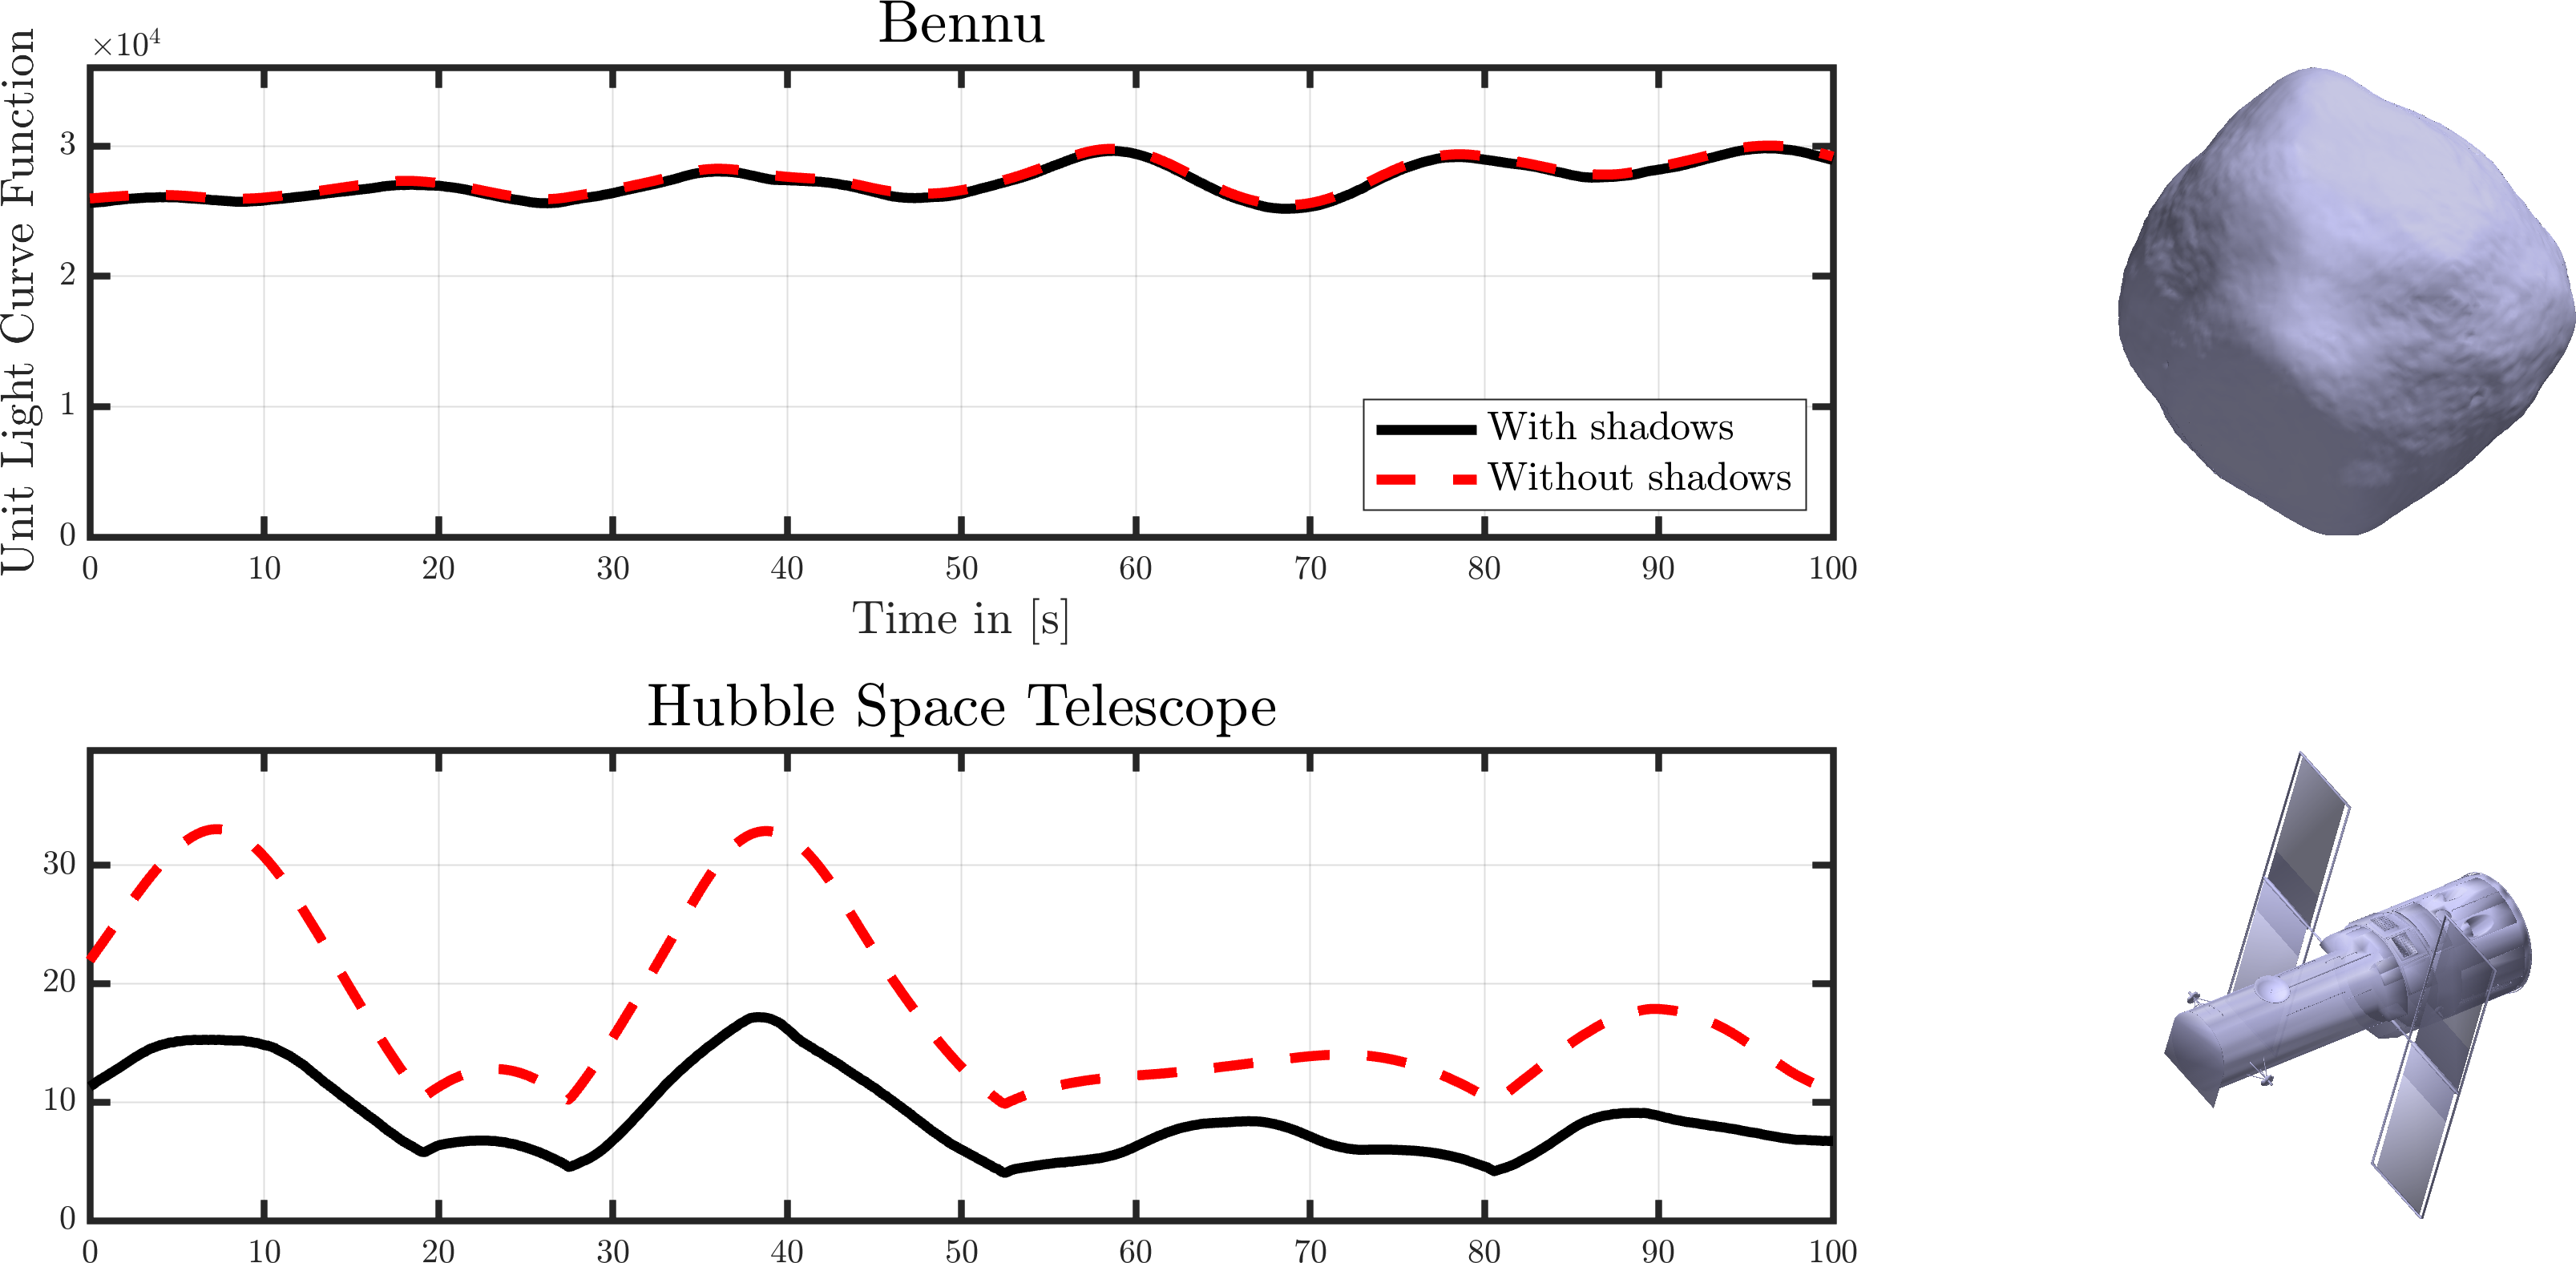
\includegraphics[width=350px]{convex_vs_nconv_lcs.png}
  \caption{Brightness errors introduced by neglecting shadows for Bennu and HST. Models from \cite{nasa_models}}
  \label{fig:hst_bennu_shadows}
\end{figure}

\subsection{Shadow Mapping for Light Curve Simulation}

\begin{figure}[!htb]
  \centering
  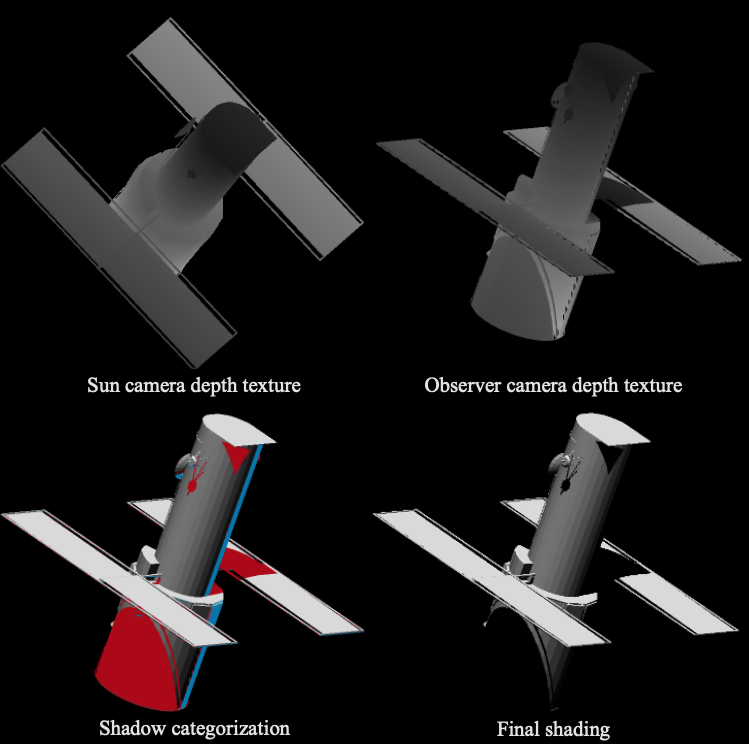
\includegraphics[width=200px]{hst_shadow_mapping/hst_shadow_mapping.png}
  \caption{Hubble Space Telescope shadow mapping with self (red) and horizon (blue) shadows rendered. Models from \cite{nasa_models}}
  \label{fig:hst_shadows_map}
\end{figure}

Given an observer and Sun vector in the body frame of the object, shadow mapping proceeds in a four step process. In step one, a camera is positioned along the Sun vector and a perpendicular depth texture is computed. In the second step, depth values in Sun camera space are transformed to observer camera space, forming a second depth texture. This second texture is used to find the closest fragment along each ray to the Sun, determining the self-shadowing condition \cite{brabec2002}. Self-shadowed fragments are classified as those further from the Sun than the closest fragment along the same ray, indicated in red in Figure \ref{fig:hst_shadows_map}. Fragments that do not pass the convex shadowing condition are horizon shadowed, indicated in blue in Figure \ref{fig:hst_shadows_map}. All remaining fragments are shaded with using the same Lambertian reflection model in \ref{lc_func_diffuse}. Computing the light curve function for the final rendered image requires summing all pixel values and dimensionalizing the result by the area of the observer camera's field of view. The light curve simulation environment used in this work was implemented in C and OpenGL using raylib \cite{raylib}.
